\documentclass{article}
\usepackage{graphicx}
\usepackage{xcolor}
\usepackage{colortbl}
\usepackage{float}
\usepackage[T1]{fontenc}

\title{Raport Plagiat}
\date{}

\begin{document}

\maketitle

\begin{center}
    \textbf{Data:} 27.01.2025 \\
    \textbf{Czas:} 23:14 \\
    \textbf{Nazwa testowanego pliku:} C:/Users/NowyLOMBARD/Desktop/Kasia/Studia/Inzynieria/PrzetworzoneDane/plikiLatex/md4 rekurencja.tex
\end{center}

\section{Inforacje ogólne dotyczące testu}

\textbf{Wynik procentowy:} 0.9975306098921257

\textbf{Czas trwania testu:} 5.125178098678589

\textbf{Liczna elementów w teście:} Input-nr-6


\section{Images}

Below is an image that is placed here using the \texttt{[H]} option to force the image placement.

\begin{figure}[H]
\centering
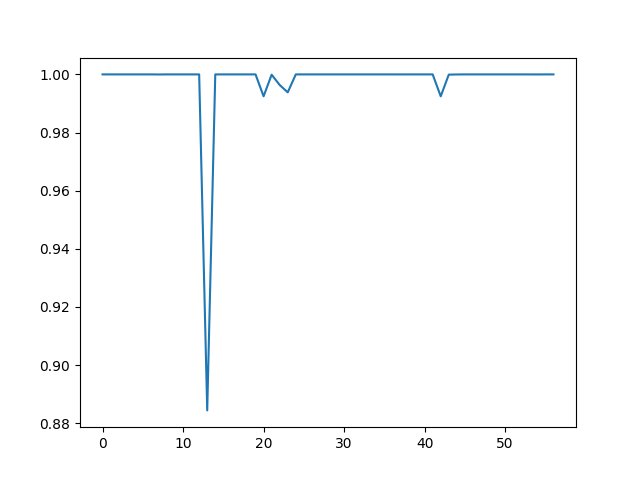
\includegraphics[width=1\textwidth]{ elements/plot0.png }
\caption{An example image}
\end{figure}

\section{Highlighted Text}

\begin{figure}[H]
\centering
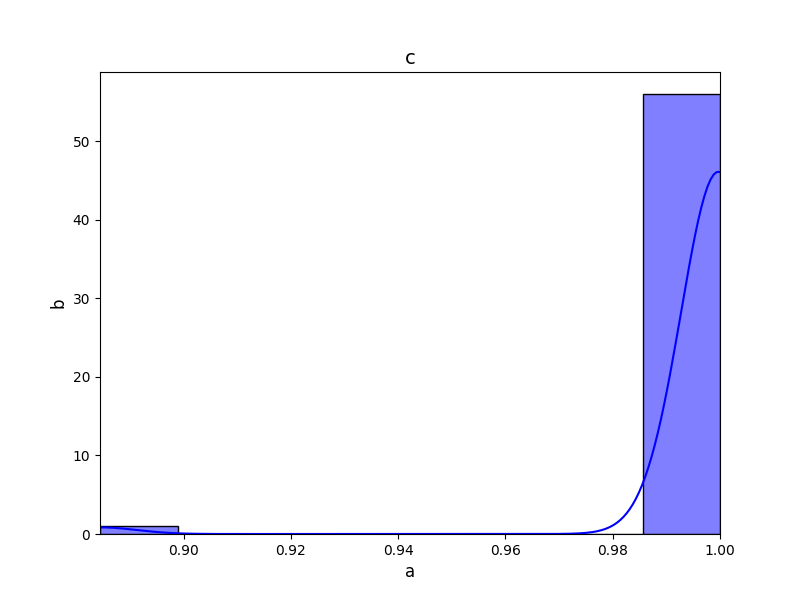
\includegraphics[width=1\textwidth]{ elements/plot1.png }
\caption{An example image}
\end{figure}




\end{document}
